% Options for packages loaded elsewhere
\PassOptionsToPackage{unicode}{hyperref}
\PassOptionsToPackage{hyphens}{url}
%
\documentclass[
]{article}
\usepackage{amsmath,amssymb}
\usepackage{lmodern}
\usepackage{iftex}
\ifPDFTeX
  \usepackage[T1]{fontenc}
  \usepackage[utf8]{inputenc}
  \usepackage{textcomp} % provide euro and other symbols
\else % if luatex or xetex
  \usepackage{unicode-math}
  \defaultfontfeatures{Scale=MatchLowercase}
  \defaultfontfeatures[\rmfamily]{Ligatures=TeX,Scale=1}
\fi
% Use upquote if available, for straight quotes in verbatim environments
\IfFileExists{upquote.sty}{\usepackage{upquote}}{}
\IfFileExists{microtype.sty}{% use microtype if available
  \usepackage[]{microtype}
  \UseMicrotypeSet[protrusion]{basicmath} % disable protrusion for tt fonts
}{}
\makeatletter
\@ifundefined{KOMAClassName}{% if non-KOMA class
  \IfFileExists{parskip.sty}{%
    \usepackage{parskip}
  }{% else
    \setlength{\parindent}{0pt}
    \setlength{\parskip}{6pt plus 2pt minus 1pt}}
}{% if KOMA class
  \KOMAoptions{parskip=half}}
\makeatother
\usepackage{xcolor}
\usepackage[margin=1in]{geometry}
\usepackage{color}
\usepackage{fancyvrb}
\newcommand{\VerbBar}{|}
\newcommand{\VERB}{\Verb[commandchars=\\\{\}]}
\DefineVerbatimEnvironment{Highlighting}{Verbatim}{commandchars=\\\{\}}
% Add ',fontsize=\small' for more characters per line
\usepackage{framed}
\definecolor{shadecolor}{RGB}{248,248,248}
\newenvironment{Shaded}{\begin{snugshade}}{\end{snugshade}}
\newcommand{\AlertTok}[1]{\textcolor[rgb]{0.94,0.16,0.16}{#1}}
\newcommand{\AnnotationTok}[1]{\textcolor[rgb]{0.56,0.35,0.01}{\textbf{\textit{#1}}}}
\newcommand{\AttributeTok}[1]{\textcolor[rgb]{0.77,0.63,0.00}{#1}}
\newcommand{\BaseNTok}[1]{\textcolor[rgb]{0.00,0.00,0.81}{#1}}
\newcommand{\BuiltInTok}[1]{#1}
\newcommand{\CharTok}[1]{\textcolor[rgb]{0.31,0.60,0.02}{#1}}
\newcommand{\CommentTok}[1]{\textcolor[rgb]{0.56,0.35,0.01}{\textit{#1}}}
\newcommand{\CommentVarTok}[1]{\textcolor[rgb]{0.56,0.35,0.01}{\textbf{\textit{#1}}}}
\newcommand{\ConstantTok}[1]{\textcolor[rgb]{0.00,0.00,0.00}{#1}}
\newcommand{\ControlFlowTok}[1]{\textcolor[rgb]{0.13,0.29,0.53}{\textbf{#1}}}
\newcommand{\DataTypeTok}[1]{\textcolor[rgb]{0.13,0.29,0.53}{#1}}
\newcommand{\DecValTok}[1]{\textcolor[rgb]{0.00,0.00,0.81}{#1}}
\newcommand{\DocumentationTok}[1]{\textcolor[rgb]{0.56,0.35,0.01}{\textbf{\textit{#1}}}}
\newcommand{\ErrorTok}[1]{\textcolor[rgb]{0.64,0.00,0.00}{\textbf{#1}}}
\newcommand{\ExtensionTok}[1]{#1}
\newcommand{\FloatTok}[1]{\textcolor[rgb]{0.00,0.00,0.81}{#1}}
\newcommand{\FunctionTok}[1]{\textcolor[rgb]{0.00,0.00,0.00}{#1}}
\newcommand{\ImportTok}[1]{#1}
\newcommand{\InformationTok}[1]{\textcolor[rgb]{0.56,0.35,0.01}{\textbf{\textit{#1}}}}
\newcommand{\KeywordTok}[1]{\textcolor[rgb]{0.13,0.29,0.53}{\textbf{#1}}}
\newcommand{\NormalTok}[1]{#1}
\newcommand{\OperatorTok}[1]{\textcolor[rgb]{0.81,0.36,0.00}{\textbf{#1}}}
\newcommand{\OtherTok}[1]{\textcolor[rgb]{0.56,0.35,0.01}{#1}}
\newcommand{\PreprocessorTok}[1]{\textcolor[rgb]{0.56,0.35,0.01}{\textit{#1}}}
\newcommand{\RegionMarkerTok}[1]{#1}
\newcommand{\SpecialCharTok}[1]{\textcolor[rgb]{0.00,0.00,0.00}{#1}}
\newcommand{\SpecialStringTok}[1]{\textcolor[rgb]{0.31,0.60,0.02}{#1}}
\newcommand{\StringTok}[1]{\textcolor[rgb]{0.31,0.60,0.02}{#1}}
\newcommand{\VariableTok}[1]{\textcolor[rgb]{0.00,0.00,0.00}{#1}}
\newcommand{\VerbatimStringTok}[1]{\textcolor[rgb]{0.31,0.60,0.02}{#1}}
\newcommand{\WarningTok}[1]{\textcolor[rgb]{0.56,0.35,0.01}{\textbf{\textit{#1}}}}
\usepackage{graphicx}
\makeatletter
\def\maxwidth{\ifdim\Gin@nat@width>\linewidth\linewidth\else\Gin@nat@width\fi}
\def\maxheight{\ifdim\Gin@nat@height>\textheight\textheight\else\Gin@nat@height\fi}
\makeatother
% Scale images if necessary, so that they will not overflow the page
% margins by default, and it is still possible to overwrite the defaults
% using explicit options in \includegraphics[width, height, ...]{}
\setkeys{Gin}{width=\maxwidth,height=\maxheight,keepaspectratio}
% Set default figure placement to htbp
\makeatletter
\def\fps@figure{htbp}
\makeatother
\setlength{\emergencystretch}{3em} % prevent overfull lines
\providecommand{\tightlist}{%
  \setlength{\itemsep}{0pt}\setlength{\parskip}{0pt}}
\setcounter{secnumdepth}{-\maxdimen} % remove section numbering
\ifLuaTeX
  \usepackage{selnolig}  % disable illegal ligatures
\fi
\IfFileExists{bookmark.sty}{\usepackage{bookmark}}{\usepackage{hyperref}}
\IfFileExists{xurl.sty}{\usepackage{xurl}}{} % add URL line breaks if available
\urlstyle{same} % disable monospaced font for URLs
\hypersetup{
  pdftitle={Reproducible Research: Peer Assessment 1},
  hidelinks,
  pdfcreator={LaTeX via pandoc}}

\title{Reproducible Research: Peer Assessment 1}
\author{}
\date{\vspace{-2.5em}}

\begin{document}
\maketitle

\hypertarget{download-and-preprocessing-the-data}{%
\subsection{Download and preprocessing the
data}\label{download-and-preprocessing-the-data}}

First, load the packages needed for the analysis.

\begin{Shaded}
\begin{Highlighting}[]
\FunctionTok{library}\NormalTok{(dplyr)}
\end{Highlighting}
\end{Shaded}

\begin{verbatim}
## Warning: package 'dplyr' was built under R version 4.2.2
\end{verbatim}

\begin{verbatim}
## 
## Attaching package: 'dplyr'
\end{verbatim}

\begin{verbatim}
## The following objects are masked from 'package:stats':
## 
##     filter, lag
\end{verbatim}

\begin{verbatim}
## The following objects are masked from 'package:base':
## 
##     intersect, setdiff, setequal, union
\end{verbatim}

\begin{Shaded}
\begin{Highlighting}[]
\FunctionTok{library}\NormalTok{(tidyr)}
\end{Highlighting}
\end{Shaded}

\begin{verbatim}
## Warning: package 'tidyr' was built under R version 4.2.2
\end{verbatim}

\begin{Shaded}
\begin{Highlighting}[]
\FunctionTok{library}\NormalTok{(lattice)}
\end{Highlighting}
\end{Shaded}

Then load the data.

\begin{Shaded}
\begin{Highlighting}[]
\FunctionTok{unzip}\NormalTok{(}\StringTok{"activity.zip"}\NormalTok{)}
\NormalTok{dat }\OtherTok{\textless{}{-}} \FunctionTok{read.csv}\NormalTok{(}\StringTok{"activity.csv"}\NormalTok{)}
\end{Highlighting}
\end{Shaded}

The format of the ``date'' column should be changed from character to
date format.

\begin{Shaded}
\begin{Highlighting}[]
\NormalTok{dat}\SpecialCharTok{$}\NormalTok{date }\OtherTok{\textless{}{-}} \FunctionTok{as.Date}\NormalTok{(dat}\SpecialCharTok{$}\NormalTok{date, }\AttributeTok{format =} \StringTok{"\%Y{-}\%m{-}\%d"}\NormalTok{)}
\end{Highlighting}
\end{Shaded}

\hypertarget{what-is-mean-total-number-of-steps-taken-per-day}{%
\subsection{What is mean total number of steps taken per
day?}\label{what-is-mean-total-number-of-steps-taken-per-day}}

First, calculate the total number of steps taken per day, ignoring
missing values in the data set for now.

\begin{Shaded}
\begin{Highlighting}[]
\NormalTok{totalPerDay }\OtherTok{\textless{}{-}}\NormalTok{ dat }\SpecialCharTok{\%\textgreater{}\%}
                \FunctionTok{subset}\NormalTok{(steps }\SpecialCharTok{!=} \StringTok{"NA"}\NormalTok{) }\SpecialCharTok{\%\textgreater{}\%}
                \FunctionTok{group\_by}\NormalTok{(date) }\SpecialCharTok{\%\textgreater{}\%}
                \FunctionTok{summarize\_at}\NormalTok{(}\StringTok{"steps"}\NormalTok{, sum)}
\end{Highlighting}
\end{Shaded}

The histogram below shows the total number of steps taken each day.

\begin{Shaded}
\begin{Highlighting}[]
\FunctionTok{hist}\NormalTok{(totalPerDay}\SpecialCharTok{$}\NormalTok{steps, }\AttributeTok{breaks =} \DecValTok{100}\NormalTok{, }\AttributeTok{xlab =} \StringTok{"Steps Range"}\NormalTok{, }
     \AttributeTok{main =} \StringTok{"Histogram of Total Steps Per Day"}\NormalTok{, }\AttributeTok{col =} \StringTok{"black"}\NormalTok{)}
\end{Highlighting}
\end{Shaded}

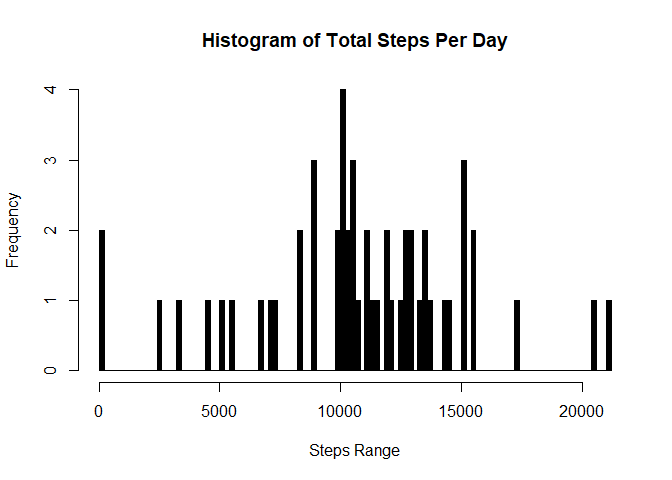
\includegraphics{PA1_template_files/figure-latex/totalPerDayhist-1.pdf}

The mean and median of the total number of steps taken per day are:

\begin{Shaded}
\begin{Highlighting}[]
\FunctionTok{mean}\NormalTok{(totalPerDay}\SpecialCharTok{$}\NormalTok{steps)}
\end{Highlighting}
\end{Shaded}

\begin{verbatim}
## [1] 10766.19
\end{verbatim}

\begin{Shaded}
\begin{Highlighting}[]
\FunctionTok{median}\NormalTok{(totalPerDay}\SpecialCharTok{$}\NormalTok{steps)}
\end{Highlighting}
\end{Shaded}

\begin{verbatim}
## [1] 10765
\end{verbatim}

\hypertarget{what-is-the-average-daily-activity-pattern}{%
\subsection{What is the average daily activity
pattern?}\label{what-is-the-average-daily-activity-pattern}}

The average daily pattern can be shown using a time series plot
(i.e.~type = ``1'') of the 5-minute interval (x-axis) and the average
number of steps taken, averaged across all days (y-axis)

\begin{Shaded}
\begin{Highlighting}[]
\NormalTok{avgPerInterval }\OtherTok{\textless{}{-}}\NormalTok{ dat }\SpecialCharTok{\%\textgreater{}\%}
                \FunctionTok{subset}\NormalTok{(steps }\SpecialCharTok{!=} \StringTok{"NA"}\NormalTok{) }\SpecialCharTok{\%\textgreater{}\%}
                \FunctionTok{group\_by}\NormalTok{(interval) }\SpecialCharTok{\%\textgreater{}\%}
                \FunctionTok{summarize\_at}\NormalTok{(}\StringTok{"steps"}\NormalTok{, mean)}

\FunctionTok{plot}\NormalTok{(avgPerInterval}\SpecialCharTok{$}\NormalTok{interval, avgPerInterval}\SpecialCharTok{$}\NormalTok{steps, }\AttributeTok{type =} \StringTok{"l"}\NormalTok{, }
     \AttributeTok{xlab =} \StringTok{"Interval"}\NormalTok{, }\AttributeTok{ylab =} \StringTok{"Steps"}\NormalTok{, }
     \AttributeTok{main =} \StringTok{"Average Number of Steps per 5{-}Minute Interval"}\NormalTok{)}
\end{Highlighting}
\end{Shaded}

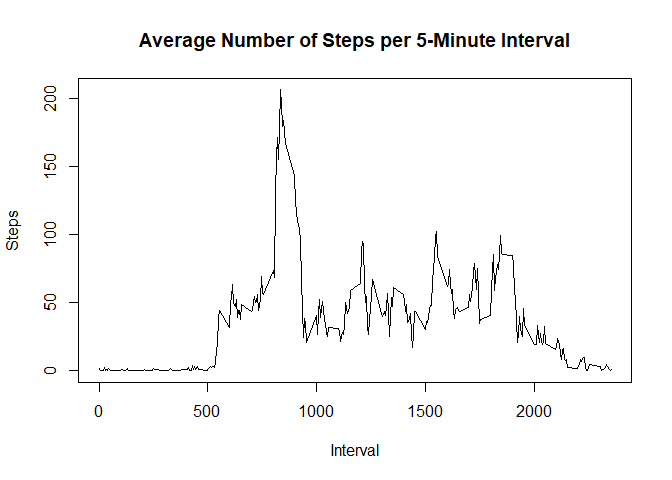
\includegraphics{PA1_template_files/figure-latex/avgPerInterval-1.pdf}

The 5-minute interval, on average across all the days in the dataset,
contains the maximum number of steps is calculated to be:

\begin{Shaded}
\begin{Highlighting}[]
\NormalTok{intervalMax }\OtherTok{\textless{}{-}} \FunctionTok{subset}\NormalTok{(avgPerInterval, avgPerInterval}\SpecialCharTok{$}\NormalTok{steps }\SpecialCharTok{==} \FunctionTok{max}\NormalTok{(avgPerInterval}\SpecialCharTok{$}\NormalTok{steps))}
\NormalTok{intervalMax}\SpecialCharTok{$}\NormalTok{interval}
\end{Highlighting}
\end{Shaded}

\begin{verbatim}
## [1] 835
\end{verbatim}

\hypertarget{imputing-missing-values}{%
\subsection{Imputing missing values}\label{imputing-missing-values}}

There are a number of days/intervals where there are missing values
(coded as NA). The presence of missing days may introduce bias into some
calculations or summaries of data. We can find out whether there are
biases by imputing the missing values and comparing the mean and median
between the two data sets.

First, find the total number of missing values in the data set (i.e.~the
total number of rows with NAs).

\begin{Shaded}
\begin{Highlighting}[]
\FunctionTok{sum}\NormalTok{(}\FunctionTok{is.na}\NormalTok{(dat}\SpecialCharTok{$}\NormalTok{steps))}
\end{Highlighting}
\end{Shaded}

\begin{verbatim}
## [1] 2304
\end{verbatim}

To impute the missing variables, Fill in NAs using the mean for the
missing 5-minute interval.

\begin{Shaded}
\begin{Highlighting}[]
\NormalTok{dat\_noNA }\OtherTok{\textless{}{-}} \FunctionTok{data.frame}\NormalTok{(}\AttributeTok{steps =} \FunctionTok{integer}\NormalTok{(}\DecValTok{0}\NormalTok{), }\AttributeTok{date =} \FunctionTok{character}\NormalTok{(}\DecValTok{0}\NormalTok{), }\AttributeTok{interval =} \FunctionTok{integer}\NormalTok{(}\DecValTok{0}\NormalTok{))}
\ControlFlowTok{for}\NormalTok{ (i }\ControlFlowTok{in} \DecValTok{1}\SpecialCharTok{:}\DecValTok{17568}\NormalTok{) \{}
\NormalTok{        dat\_noNA }\OtherTok{\textless{}{-}} \FunctionTok{rbind}\NormalTok{(dat\_noNA, dat[i, ])}
        \ControlFlowTok{if}\NormalTok{ (}\FunctionTok{is.na}\NormalTok{(dat\_noNA}\SpecialCharTok{$}\NormalTok{steps[i])) \{}
\NormalTok{                dat\_interval }\OtherTok{\textless{}{-}} \FunctionTok{subset}\NormalTok{(dat, interval }\SpecialCharTok{==}\NormalTok{ dat\_noNA}\SpecialCharTok{$}\NormalTok{interval[i])}
\NormalTok{                dat\_noNA}\SpecialCharTok{$}\NormalTok{steps[i] }\OtherTok{\textless{}{-}} \FunctionTok{mean}\NormalTok{(dat\_interval}\SpecialCharTok{$}\NormalTok{steps, }\AttributeTok{na.rm =} \ConstantTok{TRUE}\NormalTok{)}
\NormalTok{        \}}
\NormalTok{\}}
\end{Highlighting}
\end{Shaded}

The histogram below shows the total number of steps taken each day with
imputed missing values.

\begin{Shaded}
\begin{Highlighting}[]
\NormalTok{totalPerDay\_noNA }\OtherTok{\textless{}{-}}\NormalTok{ dat\_noNA }\SpecialCharTok{\%\textgreater{}\%}
        \FunctionTok{subset}\NormalTok{(steps }\SpecialCharTok{!=} \StringTok{"NA"}\NormalTok{) }\SpecialCharTok{\%\textgreater{}\%}
        \FunctionTok{group\_by}\NormalTok{(date) }\SpecialCharTok{\%\textgreater{}\%}
        \FunctionTok{summarize\_at}\NormalTok{(}\StringTok{"steps"}\NormalTok{, sum)}

\FunctionTok{hist}\NormalTok{(totalPerDay\_noNA}\SpecialCharTok{$}\NormalTok{steps, }\AttributeTok{breaks =} \DecValTok{100}\NormalTok{, }\AttributeTok{xlab =} \StringTok{"Steps Range"}\NormalTok{, }
     \AttributeTok{main =} \StringTok{"Histogram of Total Steps Per Day"}\NormalTok{, }\AttributeTok{col =} \StringTok{"black"}\NormalTok{)}
\end{Highlighting}
\end{Shaded}

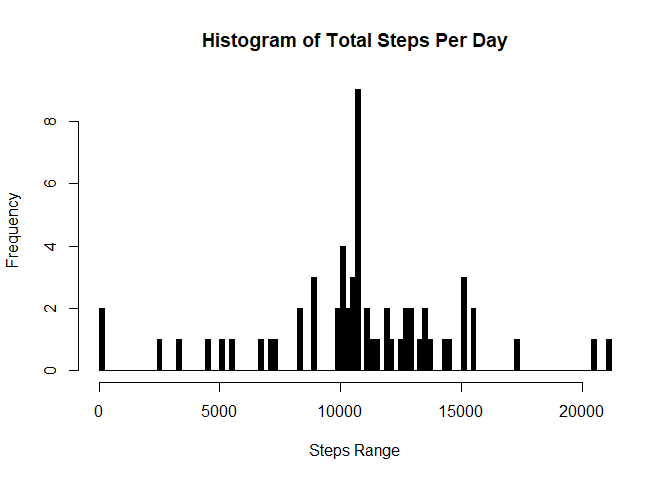
\includegraphics{PA1_template_files/figure-latex/noNAhist-1.pdf}

The mean and median of the total number of steps taken each day are:

\begin{Shaded}
\begin{Highlighting}[]
\FunctionTok{mean}\NormalTok{(totalPerDay\_noNA}\SpecialCharTok{$}\NormalTok{steps)}
\end{Highlighting}
\end{Shaded}

\begin{verbatim}
## [1] 10766.19
\end{verbatim}

\begin{Shaded}
\begin{Highlighting}[]
\FunctionTok{median}\NormalTok{(totalPerDay\_noNA}\SpecialCharTok{$}\NormalTok{steps)}
\end{Highlighting}
\end{Shaded}

\begin{verbatim}
## [1] 10766.19
\end{verbatim}

Imputing missing data on the estimates of the total daily number of
steps did not seem to impact the mean and median of the data. Therefore,
the presence of missing data did not seem to bias the calculations of
the data in the this case.

\hypertarget{are-there-differences-in-activity-patterns-between-weekdays-and-weekends}{%
\subsection{Are there differences in activity patterns between weekdays
and
weekends?}\label{are-there-differences-in-activity-patterns-between-weekdays-and-weekends}}

Create a new factor variable in the dataset with two levels -
``weekday'' and ``weekend'' indicating whether a given date is a weekday
or weekend day. We will use the data set with missing values imputed.

\begin{Shaded}
\begin{Highlighting}[]
\NormalTok{dat\_noNA}\SpecialCharTok{$}\NormalTok{day }\OtherTok{\textless{}{-}} \FunctionTok{weekdays}\NormalTok{(dat\_noNA}\SpecialCharTok{$}\NormalTok{date)}
\NormalTok{dat\_noNA}\SpecialCharTok{$}\NormalTok{day }\OtherTok{\textless{}{-}} \FunctionTok{factor}\NormalTok{(dat\_noNA}\SpecialCharTok{$}\NormalTok{day }\SpecialCharTok{==} \StringTok{"Saturday"} \SpecialCharTok{|}\NormalTok{ dat\_noNA}\SpecialCharTok{$}\NormalTok{day }\SpecialCharTok{==} \StringTok{"Sunday"}\NormalTok{, }
                       \AttributeTok{labels =} \FunctionTok{c}\NormalTok{(}\StringTok{"weekday"}\NormalTok{, }\StringTok{"weekend"}\NormalTok{))}
\end{Highlighting}
\end{Shaded}

The time series panel plot shows the 5-minute interval (x-axis) and the
average number of steps taken, averaged across all weekday days or
weekend days (y-axis).

\begin{Shaded}
\begin{Highlighting}[]
\NormalTok{avgPerInterval\_noNA }\OtherTok{\textless{}{-}}\NormalTok{ dat\_noNA }\SpecialCharTok{\%\textgreater{}\%}
                \FunctionTok{group\_by}\NormalTok{(interval, day) }\SpecialCharTok{\%\textgreater{}\%}
                \FunctionTok{summarize\_at}\NormalTok{(}\StringTok{"steps"}\NormalTok{, mean)}

\FunctionTok{xyplot}\NormalTok{(steps }\SpecialCharTok{\textasciitilde{}}\NormalTok{ interval }\SpecialCharTok{|}\NormalTok{ day, }\AttributeTok{data =}\NormalTok{ avgPerInterval\_noNA, }\AttributeTok{type =} \StringTok{"l"}\NormalTok{, }
       \AttributeTok{xlab =} \StringTok{"Interval"}\NormalTok{, }\AttributeTok{ylab =} \StringTok{"Steps"}\NormalTok{, }
       \AttributeTok{main =} \StringTok{"Average Number of Steps per 5{-}Minute Interval"}\NormalTok{, }\AttributeTok{layout =} \FunctionTok{c}\NormalTok{(}\DecValTok{1}\NormalTok{,}\DecValTok{2}\NormalTok{))}
\end{Highlighting}
\end{Shaded}

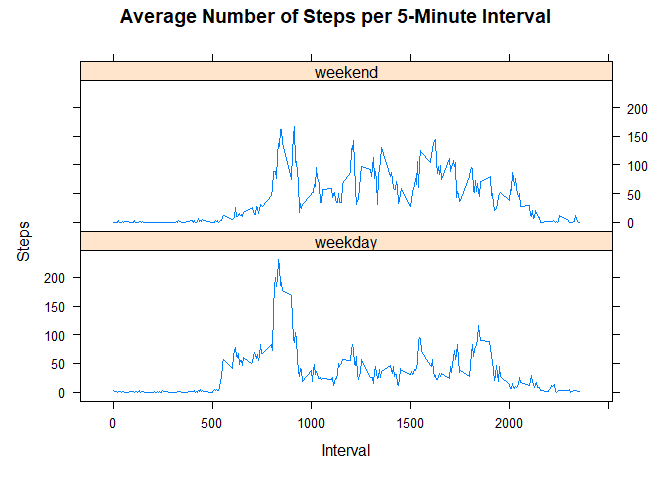
\includegraphics{PA1_template_files/figure-latex/panelPlot-1.pdf}

It can be observed that for weekdays, the number of steps do not exceed
200 in a given interval, and the pattern is consistent throughout the
day. However, on the weekends, we see a spike in number of steps between
the intervals 800-1000, and reduces for the rest of the day.

\end{document}
